\documentclass[twocolumn]{article}
\usepackage[utf8]{inputenc}
\usepackage[top=1in]{geometry}
\usepackage{graphicx}
\usepackage{booktabs}
\usepackage{amsmath,amssymb}
\usepackage{multirow}
\usepackage{hyperref}
\usepackage{xcolor}

% Calligraphic fonts
\newcommand{\calA}{{\cal A}}
\newcommand{\calB}{{\cal B}}
\newcommand{\calC}{{\cal C}}
\newcommand{\calD}{{\cal D}}
\newcommand{\calE}{{\cal E}}
\newcommand{\calF}{{\cal F}}
\newcommand{\calG}{{\cal G}}
\newcommand{\calH}{{\cal H}}
\newcommand{\calI}{{\cal I}}
\newcommand{\calJ}{{\cal J}}
\newcommand{\calK}{{\cal K}}
\newcommand{\calL}{{\cal L}}
\newcommand{\calM}{{\cal M}}
\newcommand{\calN}{{\cal N}}
\newcommand{\calO}{{\cal O}}
\newcommand{\calP}{{\cal P}}
\newcommand{\calQ}{{\cal Q}}
\newcommand{\calR}{{\cal R}}
\newcommand{\calS}{{\cal S}}
\newcommand{\calT}{{\cal T}}
\newcommand{\calU}{{\cal U}}
\newcommand{\calV}{{\cal V}}
\newcommand{\calW}{{\cal W}}
\newcommand{\calX}{{\cal X}}
\newcommand{\calY}{{\cal Y}}
\newcommand{\calZ}{{\cal Z}}

% Sets:
\newcommand{\setA}{\textsf{A}}
\newcommand{\setB}{\textsf{B}}
\newcommand{\setC}{\textsf{C}}
\newcommand{\setD}{\textsf{D}}
\newcommand{\setE}{\textsf{E}}
\newcommand{\setF}{\textsf{F}}
\newcommand{\setG}{\textsf{G}}
\newcommand{\setH}{\textsf{H}}
\newcommand{\setI}{\textsf{I}}
\newcommand{\setJ}{\textsf{J}}
\newcommand{\setK}{\textsf{K}}
\newcommand{\setL}{\textsf{L}}
\newcommand{\setM}{\textsf{M}}
\newcommand{\setN}{\textsf{N}}
\newcommand{\setO}{\textsf{O}}
\newcommand{\setP}{\textsf{P}}
\newcommand{\setQ}{\textsf{Q}}
\newcommand{\setR}{\textsf{R}}
\newcommand{\setS}{\textsf{S}}
\newcommand{\setT}{\textsf{T}}
\newcommand{\setU}{\textsf{U}}
\newcommand{\setV}{\textsf{V}}
\newcommand{\setW}{\textsf{W}}
\newcommand{\setX}{\textsf{X}}
\newcommand{\setY}{\textsf{Y}}
\newcommand{\setZ}{\textsf{Z}}

% Vectors
\newcommand{\bfa}{\mathbf{a}}
\newcommand{\bfb}{\mathbf{b}}
\newcommand{\bfc}{\mathbf{c}}
\newcommand{\bfd}{\mathbf{d}}
\newcommand{\bfe}{\mathbf{e}}
\newcommand{\bff}{\mathbf{f}}
\newcommand{\bfg}{\mathbf{g}}
\newcommand{\bfh}{\mathbf{h}}
\newcommand{\bfi}{\mathbf{i}}
\newcommand{\bfj}{\mathbf{j}}
\newcommand{\bfk}{\mathbf{k}}
\newcommand{\bfl}{\mathbf{l}}
\newcommand{\bfm}{\mathbf{m}}
\newcommand{\bfn}{\mathbf{n}}
\newcommand{\bfo}{\mathbf{o}}
\newcommand{\bfp}{\mathbf{p}}
\newcommand{\bfq}{\mathbf{q}}
\newcommand{\bfr}{\mathbf{r}}
\newcommand{\bfs}{\mathbf{s}}
\newcommand{\bft}{\mathbf{t}}
\newcommand{\bfu}{\mathbf{u}}
\newcommand{\bfv}{\mathbf{v}}
\newcommand{\bfw}{\mathbf{w}}
\newcommand{\bfx}{\mathbf{x}}
\newcommand{\bfy}{\mathbf{y}}
\newcommand{\bfz}{\mathbf{z}}


\newcommand{\bfalpha}{\boldsymbol{\alpha}}
\newcommand{\bfbeta}{\boldsymbol{\beta}}
\newcommand{\bfgamma}{\boldsymbol{\gamma}}
\newcommand{\bfdelta}{\boldsymbol{\delta}}
\newcommand{\bfepsilon}{\boldsymbol{\epsilon}}
\newcommand{\bfzeta}{\boldsymbol{\zeta}}
\newcommand{\bfeta}{\boldsymbol{\eta}}
\newcommand{\bftheta}{\boldsymbol{\theta}}
\newcommand{\bfiota}{\boldsymbol{\iota}}
\newcommand{\bfkappa}{\boldsymbol{\kappa}}
\newcommand{\bflambda}{\boldsymbol{\lambda}}
\newcommand{\bfmu}{\boldsymbol{\mu}}
\newcommand{\bfnu}{\boldsymbol{\nu}}
\newcommand{\bfomicron}{\boldsymbol{\omicron}}
\newcommand{\bfpi}{\boldsymbol{\pi}}
\newcommand{\bfrho}{\boldsymbol{\rho}}
\newcommand{\bfsigma}{\boldsymbol{\sigma}}
\newcommand{\bftau}{\boldsymbol{\tau}}
\newcommand{\bfupsilon}{\boldsymbol{\upsilon}}
\newcommand{\bfphi}{\boldsymbol{\phi}}
\newcommand{\bfchi}{\boldsymbol{\chi}}
\newcommand{\bfpsi}{\boldsymbol{\psi}}
\newcommand{\bfomega}{\boldsymbol{\omega}}
\newcommand{\bfxi}{\boldsymbol{\xi}}
\newcommand{\bfell}{\boldsymbol{\ell}}

% Matrices
\newcommand{\bfA}{\mathbf{A}}
\newcommand{\bfB}{\mathbf{B}}
\newcommand{\bfC}{\mathbf{C}}
\newcommand{\bfD}{\mathbf{D}}
\newcommand{\bfE}{\mathbf{E}}
\newcommand{\bfF}{\mathbf{F}}
\newcommand{\bfG}{\mathbf{G}}
\newcommand{\bfH}{\mathbf{H}}
\newcommand{\bfI}{\mathbf{I}}
\newcommand{\bfJ}{\mathbf{J}}
\newcommand{\bfK}{\mathbf{K}}
\newcommand{\bfL}{\mathbf{L}}
\newcommand{\bfM}{\mathbf{M}}
\newcommand{\bfN}{\mathbf{N}}
\newcommand{\bfO}{\mathbf{O}}
\newcommand{\bfP}{\mathbf{P}}
\newcommand{\bfQ}{\mathbf{Q}}
\newcommand{\bfR}{\mathbf{R}}
\newcommand{\bfS}{\mathbf{S}}
\newcommand{\bfT}{\mathbf{T}}
\newcommand{\bfU}{\mathbf{U}}
\newcommand{\bfV}{\mathbf{V}}
\newcommand{\bfW}{\mathbf{W}}
\newcommand{\bfX}{\mathbf{X}}
\newcommand{\bfY}{\mathbf{Y}}
\newcommand{\bfZ}{\mathbf{Z}}


\newcommand{\bfGamma}{\boldsymbol{\Gamma}}
\newcommand{\bfDelta}{\boldsymbol{\Delta}}
\newcommand{\bfTheta}{\boldsymbol{\Theta}}
\newcommand{\bfLambda}{\boldsymbol{\Lambda}}
\newcommand{\bfPi}{\boldsymbol{\Pi}}
\newcommand{\bfSigma}{\boldsymbol{\Sigma}}
\newcommand{\bfUpsilon}{\boldsymbol{\Upsilon}}
\newcommand{\bfPhi}{\boldsymbol{\Phi}}
\newcommand{\bfPsi}{\boldsymbol{\Psi}}
\newcommand{\bfOmega}{\boldsymbol{\Omega}}


% Blackboard Bold:
\newcommand{\bbA}{\mathbb{A}}
\newcommand{\bbB}{\mathbb{B}}
\newcommand{\bbC}{\mathbb{C}}
\newcommand{\bbD}{\mathbb{D}}
\newcommand{\bbE}{\mathbb{E}}
\newcommand{\bbF}{\mathbb{F}}
\newcommand{\bbG}{\mathbb{G}}
\newcommand{\bbH}{\mathbb{H}}
\newcommand{\bbI}{\mathbb{I}}
\newcommand{\bbJ}{\mathbb{J}}
\newcommand{\bbK}{\mathbb{K}}
\newcommand{\bbL}{\mathbb{L}}
\newcommand{\bbM}{\mathbb{M}}
\newcommand{\bbN}{\mathbb{N}}
\newcommand{\bbO}{\mathbb{O}}
\newcommand{\bbP}{\mathbb{P}}
\newcommand{\bbQ}{\mathbb{Q}}
\newcommand{\bbR}{\mathbb{R}}
\newcommand{\bbS}{\mathbb{S}}
\newcommand{\bbT}{\mathbb{T}}
\newcommand{\bbU}{\mathbb{U}}
\newcommand{\bbV}{\mathbb{V}}
\newcommand{\bbW}{\mathbb{W}}
\newcommand{\bbX}{\mathbb{X}}
\newcommand{\bbY}{\mathbb{Y}}
\newcommand{\bbZ}{\mathbb{Z}}




\title{Homework 1}
\author{Max marks: 80}
\date{Due on September 10, 2021, before class.}
\newtheorem{prob}{Problem}

\newcommand{\bx}{\bar{x}}
\newcommand{\by}{\bar{y}}
\newcommand{\bz}{\bar{z}}
\begin{document}

\maketitle

\begin{prob}
Use algebraic manipulation to find the minimum sum-of-products expression for the function $f = x_1x_3 + x_1\bx_2 + \bx_1 x_2 x_3 + \bx_1 \bx_2 \bx_3$. ~\cite[Prob 2.12]{brown2013fundamentals}[10 marks]
\end{prob}

\subsubsection*{Solution}
\begin{align}
f = x_1x_3 + x_1\bx_2 + \bx_1 x_2 x_3 + \bx_1 \bx_2 \bx_3
  \label{eq:1-src}
\end{align}

To find the minimum sum-of-products expression, we will fill the K-map step by step. $f$ has 4
terms. We will fill K-map for each term separately and then join them together
to get the full K-map.  

\begin{enumerate}
  \item 
K-map for the term $x_1x_3$ is,
\begin{tabular}{c|c|c|c|c}
  \toprule
  & \multicolumn{2}{c|}{$\bx_1$} & \multicolumn{2}{c}{$x_1$}
  \\
  & $\bx_2$ & \multicolumn{2}{c|}{$x_2$} & $\bx_2$ \\
  \midrule
  $\bx_3$ & 0 & 0 & 0 & 0\\
  \\
  $x_3$   & 0 & 0 & 1 & 1\\
  \bottomrule
\end{tabular}

\item 
K-map for the term $x_1\bx_2$ is:
\begin{tabular}{c|c|c|c|c}
  \toprule
  & \multicolumn{2}{c|}{$\bx_1$} & \multicolumn{2}{c}{$x_1$}
  \\
  & $\bx_2$ & \multicolumn{2}{c|}{$x_2$} & $\bx_2$ \\
  \midrule
  $\bx_3$ & 0 & 0 & 0 & 1\\
  \\
  $x_3$   & 0 & 0 & 0 & 1\\
  \bottomrule
\end{tabular}


\item 
K-map for the term $\bx_1x_2x_3$ is:
\begin{tabular}{c|c|c|c|c}
  \toprule
  & \multicolumn{2}{c|}{$\bx_1$} & \multicolumn{2}{c}{$x_1$}
  \\
  & $\bx_2$ & \multicolumn{2}{c|}{$x_2$} & $\bx_2$ \\
  \midrule
  $\bx_3$ & 0 & 0 & 0 & 0\\
  \\
  $x_3$   & 0 & 1 & 0 & 0\\
  \bottomrule
\end{tabular}

\item 
K-map for the term $\bx_1\bx_2\bx_3$ is:
\begin{tabular}{c|c|c|c|c}
  \toprule
  & \multicolumn{2}{c|}{$\bx_1$} & \multicolumn{2}{c}{$x_1$}
  \\
  & $\bx_2$ & \multicolumn{2}{c|}{$x_2$} & $\bx_2$ \\
  \midrule
  $\bx_3$ & 1 & 0 & 0 & 0\\
  \\
  $x_3$   & 0 & 0 & 0 & 0\\
  \bottomrule
\end{tabular}
\end{enumerate}

Taking OR of the four K-maps, we get the K-map for $f=x_1 x_3 + x_1 \bx_2 + \bx_1 x_2 x_3 + \bx_1 \bx_2 \bx_3$:
\begin{tabular}{c|c|c|c|c}
  \toprule
  & \multicolumn{2}{c|}{$\bx_1$} & \multicolumn{2}{c}{$x_1$}
  \\
  & $\bx_2$ & \multicolumn{2}{c|}{$x_2$} & $\bx_2$ \\
  \midrule
  $\bx_3$ & 1 & 0 & 0 & 1\\
  \\
  $x_3$   & 0 & 1 & 1 & 1\\
  \bottomrule
\end{tabular}

This K-map can be decomposed into the sum of three K-maps with two minterms each:
\begin{enumerate}
  \item 
\begin{tabular}{c|c|c|c|c}
  \toprule
  & \multicolumn{2}{c|}{$\bx_1$} & \multicolumn{2}{c}{$x_1$}
  \\
  & $\bx_2$ & \multicolumn{2}{c|}{$x_2$} & $\bx_2$ \\
  \midrule
  $\bx_3$ & 0 & 0 & 0 & 0\\
  \\
  $x_3$   & 0 & 1 & 1 & 0\\
  \bottomrule
\end{tabular},
\\
which corresponds to the expression, $x_2 x_3$.

\item
\begin{tabular}{c|c|c|c|c}
  \toprule
  & \multicolumn{2}{c|}{$\bx_1$} & \multicolumn{2}{c}{$x_1$}
  \\
  & $\bx_2$ & \multicolumn{2}{c|}{$x_2$} & $\bx_2$ \\
  \midrule
  $\bx_3$ & 0 & 0 & 0 & 1\\
  \\
  $x_3$   & 0 & 0 & 0 & 1\\
  \bottomrule
\end{tabular},
\\
which corresponds to the expression, $x_1 \bx_2$.

\item
\begin{tabular}{c|c|c|c|c}
  \toprule
  & \multicolumn{2}{c|}{$\bx_1$} & \multicolumn{2}{c}{$x_1$}
  \\
  & $\bx_2$ & \multicolumn{2}{c|}{$x_2$} & $\bx_2$ \\
  \midrule
  $\bx_3$ & 1 & 0 & 0 & 1\\
  \\
  $x_3$   & 0 & 0 & 0 & 0\\
  \bottomrule
\end{tabular},
\\
which corresponds to the expression, $\bx_2 \bx_3$.
\end{enumerate}

Taking the OR of previous 3 K-maps, we get the minimum SOP expression for
\begin{align}
f = x_2 x_3 + x_1 \bx_2 + \bx_2 \bx_3
  \label{eq:1-des}
\end{align}

However, this problem specifically asks for finding the minimal sum-of-products
expression \emph{using algebraic manipulation}.

From the K-map solution, we note
that the first expression $x_2x_3$ in \eqref{eq:1-des} corresponds to the region
in K-map that comes from $x_1x_3$ and $\bx_1 x_2 x_3$ in \eqref{eq:1-src}. This
means we should be able to write $x_2x_3$ from $x_1x_3 + \bx_1 x_2 x_3$.
%
\begin{align}
  &x_1x_3 + \bx_1 x_2 x_3 &
  \notag\\
  &=x_1\cdot 1 \cdot x_3 + \bx_1 x_2 x_3 & \because 1 \cdot z = z
  \notag\\
  &= x_1(x_2 + \bx_2)x_3 + \bx_1 x_2 x_3 & \because 1 = z + \bz
  \notag\\
  &= x_1x_2x_3 + x_1\bx_2x_3 + \bx_1 x_2 x_3 & \text{dist. prop.}
  \notag\\
  &= (x_1 + \bx_1)x_2x_3 + x_1\bx_2 x_3 & \text{dist. prop.}
  \notag\\
  &= x_2x_3 + x_1 \bx_2 x_3 & \because z+\bz = 1
    \label{eq:1-part1}
\end{align}
%
From the K-map solution, we also note that second term $x_1\bx_2$ need not
change. Although it can be combined with $\bx_1 \bx_2 \bx_3$ to get the third
term $\bx_2 \bx_3$ of the \eqref{eq:1-des}.
%
\begin{align}
  &x_1\bx_2 + \bx_1 \bx_2  \bx_3 &
  \notag\\
  &= x_1\bx_2 (1 + \bx_3) + \bx_1 \bx_2  \bx_3 & \because 1 + z = 1
  \notag\\
  &= x_1\bx_2 + x_1\bx_2\bx_3 + \bx_1 \bx_2 \bx_3 & \text{dist. prop.}
  \notag\\
  &= x_1\bx_2 + (x_1 + \bx_1) \bx_2 \bx_3 & \text{dist. prop.}
  \notag\\
  &= x_1\bx_2 + \bx_2 \bx_3
    \label{eq:1-part2}
\end{align}
%
Taking OR of \eqref{eq:1-part1} and \eqref{eq:1-part2}, we get $f$ on the LHS,
but on the RHS we have an additional term of $x_1 \bx_2 x_3$,
%
\begin{align}
  f = x_2 x_3 + x_1 \bx_2 x_3 + x_1 \bx_2 + \bx_2\bx_3.
  \label{eq:1-before-absorbed}
\end{align}
%
That is not a problem, because $x_1 \bx_3 x_3$ can be easily \emph{absorbed} by
$x_1 \bx_2$,
%
\begin{align}
  &x_1 \bx_2 x_3 + x_1 \bx_2
    \notag\\
  &= x_1 \bx_2 ( x_3 +  1) & \text{dist. prop.}
    \notag\\
  &= x_1 \bx_2  & \because 1 + z = 1
                  \label{eq:1-absorbed}
\end{align}
%
Putting \eqref{eq:1-absorbed} in \eqref{eq:1-before-absorbed}, we get the
desired simplest (in terms of number of inputs and number of gates) SOP expression by \emph{algebraic manipulation},
%
\begin{align}
  f = x_2 x_3 +  x_1 \bx_2 + \bx_2\bx_3.
\end{align}

\begin{prob}
Use algebraic manipulation to find the minimum sum-of-products expression for the function $f = x_1\bx_2\bx_3 + x_1x_2x_4 + x_1\bx_2 x_3\bx_4$.~\cite[Prob 2.13]{brown2013fundamentals}[10 marks]
\end{prob}

\subsubsection*{Solution}
Let's try another approach to illustrate this. This time let's color the K-maps
according the product terms. Let's assign a color to each of the terms,
%
\begin{align}
f = {\color{red}x_1\bx_2\bx_3} + {\color{blue}x_1x_2x_4} + {\color{green}x_1\bx_2 x_3\bx_4}.
  \label{eq:2-src}
\end{align}
%
This expression has 4-variables, so we need $2^{4} = 16$ cell K-map,
\\
\begin{tabular}{c|c|c|c|c|c}
  \toprule
  && \multicolumn{2}{c|}{$\bx_1$} & \multicolumn{2}{c}{$x_1$}
  \\
  && $\bx_2$ & \multicolumn{2}{c|}{$x_2$} & $\bx_2$
  \\ \midrule
  \multirow{2}{*}{$\bx_3$} & $\bx_4$
                                  & 0 & 0 & 0 & {\color{red}1}
  \\
  & $x_4$
                                  & 0 & 0 & {\color{blue}1} & {\color{red}1}
  \\
  \multirow{2}{*}{$x_3$}   &  $x_4$
                                  & 0 & 0 & {\color{blue}1} & 0
  \\
  & $\bx_4$
                                  & 0 & 0 & 0 & {\color{green}1}
  \\\bottomrule
\end{tabular}.
\\
The ones in the K-map are already paired-up except the green {\color{green}1},
which we can pair up with one of the top red {\color{red}1}.
\\
\begin{tabular}{c|c|c|c|c|c}
  \toprule
  && \multicolumn{2}{c|}{$\bx_1$} & \multicolumn{2}{c}{$x_1$}
  \\
  && $\bx_2$ & \multicolumn{2}{c|}{$x_2$} & $\bx_2$
  \\ \midrule
  \multirow{2}{*}{$\bx_3$} & $\bx_4$
                                  & 0 & 0 & 0 & {\color{green}1}+{\color{red}1}
  \\
  & $x_4$
                                  & 0 & 0 & {\color{blue}1} & {\color{red}1}
  \\
  \multirow{2}{*}{$x_3$}   &  $x_4$
                                  & 0 & 0 & {\color{blue}1} & 0
  \\
  & $\bx_4$
                                  & 0 & 0 & 0 & {\color{green}1}
  \\\bottomrule
\end{tabular}.
\\
Here we use {\color{green}1}+{\color{red}1} to highlight that the minterm
$x_1\bx_2\bx_3\bx_4$ is paired up with two terms: green and red. Now, we can read the K-map
into an expression,
\begin{align}
  f = {\color{red}x_1\bx_2\bx_3} + {\color{blue}x_1x_2x_4} + {\color{green}x_1\bx_2\bx_4}
\end{align}

To derive the same result from \emph{algebraic manipulation}, it is clear that
we only need to manipulate the red and green terms; the blue term stays untouched.
%
\begin{align}
& {\color{red}x_1\bx_2\bx_3} +  {\color{green}x_1\bx_2x_3\bx_4} &
  \notag\\
  &= {\color{red}x_1\bx_2\bx_3 (1 + \bx_4)} +  {\color{green}x_1\bx_2x_3\bx_4} & \because 1 = 1 + z
  \notag\\
  &= {\color{red}x_1\bx_2\bx_3 } + x_1\bx_2\bx_3\bx_4 + {\color{green}x_1\bx_2x_3\bx_4} & \text{dist. prop.}
  \notag\\
  &= {\color{red}x_1\bx_2\bx_3 } + {\color{green}x_1\bx_2(\bx_3 + x_3)\bx_4 } & \text{dist. prop.}.
  \notag\\
  &= {\color{red}x_1\bx_2\bx_3 } + {\color{green}x_1\bx_2\bx_4 } & \because z + \bz = 1
                                                                   \label{eq:2-part1}
\end{align}
%
Putting \eqref{eq:2-part1} in \eqref{eq:2-src}, we get,
%
\begin{align}
  f = {\color{red}x_1\bx_2\bx_3} + {\color{blue}x_1x_2x_4} + {\color{green}x_1\bx_2\bx_4},
\end{align}
%
which is the simplest SOP expression.
  

\begin{figure}
\centering
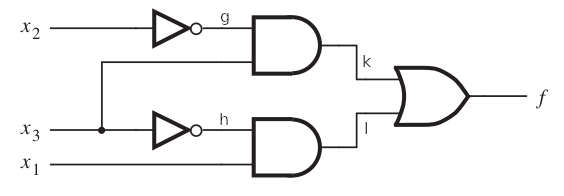
\includegraphics[width=\linewidth]{fig-2.24a.png}
\caption{A three-input circuit}
\label{fig:fig-2.24a}
\end{figure}

\begin{figure}
    \centering
    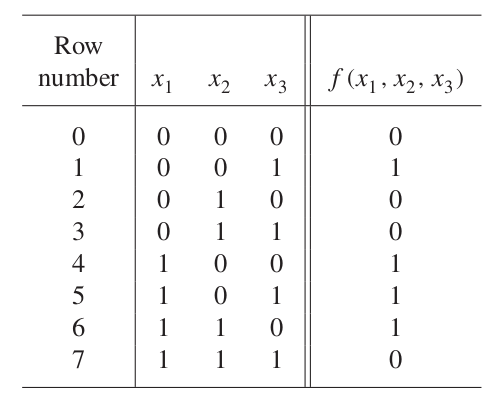
\includegraphics[width=\linewidth]{fig-2.23.png}
    \caption{A three-variable function}
    \label{fig:fig-2.23}
\end{figure}


\begin{prob}
Draw a timing diagram for the circuit in Figure~\ref{fig:fig-2.24a}. Show the
waveforms that can be observed on all wires (f, g, h, k, l) in the circuit.\cite[Prob 2.8]{brown2013fundamentals}[10 marks]
\end{prob}
\subsubsection*{Solution}
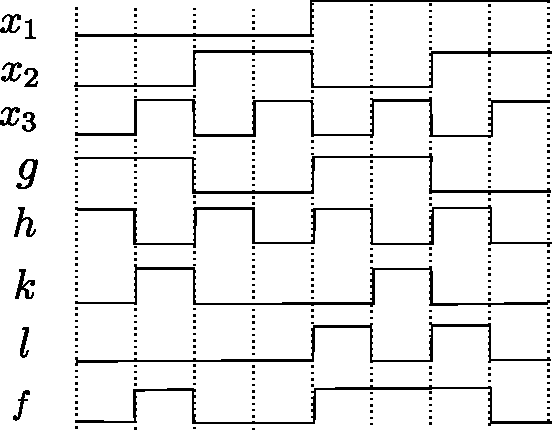
\includegraphics[width=\linewidth]{fig/timing-diagram.pdf}

\begin{prob}
Represent the function in Figure~\ref{fig:fig-2.23} in the form of a Venn diagram and find its minimal
sum-of-products form.~\cite[Prob 2.17]{brown2013fundamentals}[10 marks]
\end{prob}
\subsubsection*{Solution}
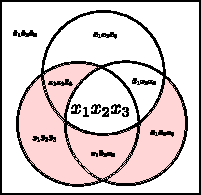
\includegraphics[width=\linewidth]{fig/venn-diagram.pdf}

Minimal SOP form is,
\[
f = x_1 \bx_3 + \bx_2 x_3
\]

\begin{prob}
Use algebraic manipulation to prove that $(x+y)\cdot(x+\bar{y}) = x$. \cite[Prob 2.2]{brown2013fundamentals} [10 marks].
\end{prob}
\subsubsection*{Solution}

\begin{align}
  \text{LHS} &= (x+y)cdot(x+\bar{y}) &
                                       \notag\\
             &= (x+y)x + (x+y)\by & \text{dist. prop.}
                                    \notag\\
             &= x \cdot x + yx + x\by + y\cdot \by & \text{dist. prop.}
                                                     \notag\\
             &= x + yx + x\by + 0 & \because y \cdot \by = 0
                                    \notag\\
             &= x(1+y +\by) & \text{dist. prop.}
                              \notag \\
             &= x\cdot 1 & \because 1 + z = 1
                           \notag \\
             &= x = \text{RHS}& \because x \cdot 1 = x
\end{align}


\begin{prob}
  Determine whether or not the following expressions are valid, i.e., whether the left- and
  right-hand sides represent the same function.
  \cite[Prob 2.7]{brown2013fundamentals}[10 marks]
  \begin{enumerate}
  \item $x_1 \bx_3 + x_2 x_3 + \bx_2 \bx_3 = (\bx_1 + \bx_2 + x_3)(x_1 + x_2 + \bx_3)(\bx_1 + x_2 + \bx_3)$
  \item $(x_1 + x_3)(\bx_1 + \bx_2 + \bx_3)(\bx_1 + x_2) = (x_1 + x_2)(x_2 + x_3)(\bx_1 + \bx_3)$
    \end{enumerate}
\end{prob}

\subsubsection*{Solution 6.1}
    \begin{align*}
      \text{LHS} &= x_1 \bx_3 + x_2 x_3 + \bx_2 \bx_3
      \\
                 &= x_1 (x_2 + \bx_2) \bx_3 + (x_1 + \bx_1)x_2 x_3
                   \\
                 &\qquad+ (x_1 + \bx_1)\bx_2 \bx_3
      \\
                 &= x_1 x_2\bx_3 + x_1\bx_2 \bx_3 + x_1x_2x_3 + \bx_1x_2 x_3 \\
      &\qquad + x_1\bx_2\bx_3 + \bx_1\bx_2 \bx_3
        \\
      &= \sum m(6, 4, 7, 3, 4, 0) = \sum m(0, 3, 4, 6, 7)
      \end{align*}

    \begin{align*}
      \text{RHS} &= (\bx_1 + \bx_2 + x_3)(x_1 + x_2 + \bx_3)(\bx_1 + x_2 + \bx_3)
      \\
                 &= \prod M(6, 1, 5)
      \\
      &= \sum m(0, 2, 3, 4, 7)
    \end{align*}
    Since LHS $\ne$ RHS, hence the expression (1) is not valid.

\subsubsection*{Solution 6.2}
Take the inversion of both sides of the equation, (2) is valid if and only if
%
\begin{align*}
  &\overline{(x_1 + x_3)(\bx_1 + \bx_2 + \bx_3)(\bx_1 + x_2)}
  \\
  &\qquad = \overline{(x_1 + x_2)(x_2 + x_3)(\bx_1 + \bx_3)}.
  \\
  &\text{ or } \bx_1\bx_3 + x_1x_2x_3 + x_1\bx_2 = \bx_1\bx_2 + \bx_2\bx_3 + x_1x_3
\end{align*}%
% 
%
\begin{align*}
\text{LHS} &= \bx_1\bx_3 + x_1x_2x_3 + x_1\bx_2
  \\
           &= \bx_1 (x_2 + \bx_2)\bx_3 + x_1x_2x_3 + x_1\bx_2(x_3 + \bx_3)
  \\
           &= \bx_1 x_2\bx_3 + \bx_1\bx_2 \bx_3 + x_1 x_2 x_3 + x_1 \bx_2 x_3
  \\
             &\qquad + x_1\bx_2 \bx_3
  \\
           &= \sum m(2, 0, 7, 5, 4) = \sum m(0, 2, 4, 5, 7)
\end{align*}%
% 
%
\begin{align*}
\text{RHS} &= \bx_1 \bx_2 + \bx_2 \bx_3 + x_1 x_3
  \\
           &= \bx_1 \bx_2 (x_3 + \bx_3) + (x_1 + \bx_1) \bx_2 \bx_3
  \\
  &\qquad + x_1 (x_2 + \bx_2) x_3
  \\
           &= \bx_1 \bx_2 x_3 + \bx_1 \bx_2 \bx_3 + x_1 \bx_2 \bx_3 + \bx_1 \bx_2 \bx_3
  \\
  &\qquad + x_1 x_2 x_3 + x_1 \bx_2 x_3
  \\
           &= \sum m(1, 0, 4, 0, 7, 5)
\end{align*}%
% 
Since LHS $\ne$ RHS the expression is not valid.


\begin{prob}
Design the simplest sum-of-products circuit that implements the function $f (x_1 , x_2 , x_3 ) = \sum m(3, 4, 6, 7)$.~\cite[Prob 2.21]{brown2013fundamentals}[10 marks]
\end{prob}
\subsubsection*{Solution}

\begin{tabular}{c|c|c|c|c}
  \toprule
  & \multicolumn{2}{c|}{$\bx_1$} & \multicolumn{2}{c}{$x_1$}
  \\
  & $\bx_2$ & \multicolumn{2}{c|}{$x_2$} & $\bx_2$
  \\ \midrule
  $\bx_3$ & 0 & 0 & {\color{green}1} & {\color{green}1}
  \\
  $x_3$ & 0 & {\color{red}1} & {\color{red}1} & 0
  \\\bottomrule
\end{tabular}.
\\
Simplest SOP expression is, $f(x_1, x_2, x_3) = {\color{green}x_1 \bx_3} +
{\color{red}x_2 x_3} $.

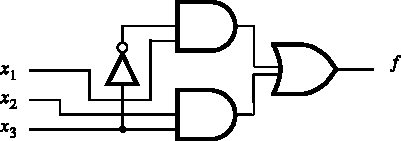
\includegraphics[width=\linewidth]{fig/prob-7-sop-circuit.pdf}

\begin{prob}
Design the simplest product-of-sums circuit that implements the function $f (x_1 , x_2 , x_3 ) = \prod M (0, 2, 5)$.~\cite[Prob 2.22]{brown2013fundamentals}[10 marks]
\end{prob}
\subsubsection*{Solution}
\begin{align}
\bar{f}(x_1, x_2, x_3) = \sum m(0, 2, 5)
\end{align}

The K-map is for $\bar{f}$ is:
\begin{tabular}{c|c|c|c|c}
  \toprule
  & \multicolumn{2}{c|}{$\bx_1$} & \multicolumn{2}{c}{$x_1$}
  \\
  & $\bx_2$ & \multicolumn{2}{c|}{$x_2$} & $\bx_2$
  \\ \midrule
  $\bx_3$ & {\color{red}1} & {\color{red}1} & 0 & 0
  \\
  $x_3$ & 0 & 0 & 0 & {\color{green}1}
  \\\bottomrule
\end{tabular}.
\\
Simplest SOP expression for $\bar{f}(x_1, x_2, x_3) = {\color{red}\bx_1 \bx_3} + {\color{green}x_1\bx_2 x_3}$.

By DeMorgan's theorem, we get the simplest POS expression is, $f(x_1, x_2, x_3) = {\color{red}(x_1 + x_3)}{\color{green}(\bx_1 + x_2 + \bx_3)} $.

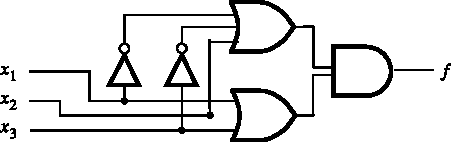
\includegraphics[width=\linewidth]{fig/prob-8-pos-circuit.pdf}


\bibliography{main}
\bibliographystyle{plain}
\end{document}
